%\documentclass[conference]{IEEEtran}


\documentclass[twocolumn]{article}
\usepackage[utf8]{inputenc}
\usepackage{times}
\usepackage{xcolor}
\usepackage{blindtext}
\usepackage{graphicx}
\frenchspacing  
\usepackage{wrapfig}
\usepackage{textcomp}



    
    
\begin{document}

\title{A Survey on Interest Flooding Attack (IFA) Countermeasures and Mitigation in Named Data Networking (NDN)}

\author{Abdullah Abumouzah\\
Department of Engineering and Computer Science\\
University of Colorado Colorado Springs\\
Email: aabumouz@uccs.edu}





\maketitle

\begin{abstract}
\textbf{Today's internet is exposed to a lot of security breaches; one of them is denial-of-service (DoS) or distributed DoS (DDoS). Named-data networking is one the proposed architectures that promised to resolve many of today's internet limitation, including security weaknesses. NDN however is like any other architecture, has its own weaknesses and vulnerabilities. \textit{Interest flooding attack} is one of these attacks that can targeted in the NDN. It could exhaust the nodes resources in the NDN routers or producer's content. This survey illustrates the different ways of how to launch this attack and what are the proposed mitigation and countermeasures.}   

\end{abstract}

%\begin{IEEEkeywords}
\textbf{\textit{Index---Information-centric networking, Named-data networking, Interest flooding attack, Denial-of-service}}
%\end{IEEEkeywords}

%\nocite{*}
\section{Introduction}
Information-Centring-Networking is considered to be the next future internet architecture \cite{6231276}. NDN is one instance of five projects that funded by the United State National Science Foundation (NSF) under the Future Internet Architecture Program (FIA).

The early revolution of the internet has evolved the concept of the host-to-host communication using the IP address as a presenter for each host. However, with the vast extension of the internet adoption and the need for robust security, users’ requirements and the nature of the applications dispute the capability of current architecture. Thus, it has been agreed that there is a necessity to develop a different model that address all those services and can concurrently operate on the existing mediums, if possible.  

NDN took its principle from the Content-Centric Network (CCN) architecture that was publically presented in 2009 by professor Van Jacobson \cite{Jacobson:2009:NNC:1658939.1658941}. CCN was created based on the concept of the Host-Centric networking that is used on the current internet; by replacing the dependency of the IP address into the content-name on routing. NDN provides more efficiency and security assurance when sharing data over the public network. NDN abandoned the hosting entity, where users can be more concerned about data than the host of that data per se. 

Current internet has been always suffering on security, leaving many threats unsolved properly. One of these threats is the DDoS attack. Attackers, using online zombies or bots, can target a specific node or network and exhaust it with a fake packets that causes undesirable traffic. DDoS by overwhelming the network could cause a degradation on the network performance. Furthermore, it could target a specific host which could crash the CPU and shout the service down.

Although NDN provides a resilient security architecture, DDoS attacks are still applicable. Interest in NDN are recorded in the NDN through the router's Pending Interest Tables (PIT). PITs creates new entry for each interest that has no corresponding content on the Content Store (CS), and was not previously requested by another node. Routers use the PITs entries to forward back, at the same path, the retrieved data to the consumer/requester. Attackers can launch a DDoS attack on the NDN by injecting spoofed interests that would neither be satisfied in the routers nor on the end-hosts. Those spoofed interests can either overload the PIT entries in a router which eliminate the ability of the router to server any further legitimate interest. Also, this attack can be achieved by creating an non-existing interest that would be forwarded to all neighbored nodes all over the internet by the Forwarding Information Table (FIB); this approach with an excessive number of spoofed interest could cause a degradation on the network performance. This type pf attacks is named Interest Flooding Attack in the named data networking. 

in this paper, we illustrates the NDN architecture in section II. Section III explains the IFA attack. Section IV analyze the current literature. Section V provide some discussions questions. in section VI we conclude this paper.   


\section{NDN Architecture Overview}
The principle and sturdy design of the NDN architecture is a derivation from the current host-centric network architecture (IP). \cite{Pan2011}. The phenomenal design of the IP internet hourglass involves the thin waist layer which allows both the upper and lower layers to operate independently; it is however the element that causes most of the limitations of the design per se. IP architecture proposed to allow a communication network among endpoints entities that their packets could only be named digitally through the IP address. However, With the dominant growth of the digital media, e-commerce and social network there became a need to use the internet not only for network communication but for content distribution. As per Cisco white paper \cite{Cisco2015}, on 2014, the content delivery network such as Netflix, Youtube and Akamai had carried about 39\% of the global internet traffic expecting this number to grow up to 62\% on 2019.

Just because how the distribution network is more general than the communication network, it is more complex to solve distribution problems with the IP architecture proposals. NDN hourglass architecture Figure.[1] retains the internet hourglass with evolving the thin waist layer to not only containing those problems, but also providing secured and more efficient platform.

NDN architecture removes the restriction of using the endpoints as the only source to fetch or secure data. In contrast to the communication network, NDN changes the concept of relying on network services from only delivering the packets from a given node address to also being able to retrieve data that identified by a given name. Thus it serves the content distribution schemes more properly.
\begin{figure} [ht]
    \centering
    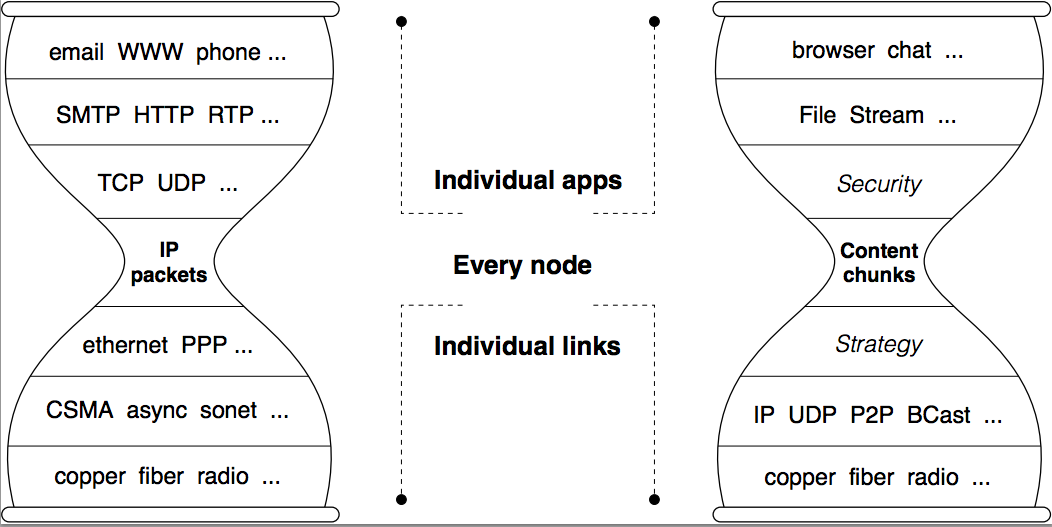
\includegraphics[width=\columnwidth]{hourglass.png}
    \caption{ \small NDN Hourglass Architecture}
    \label{fig:my_label}
\end{figure}

NDN by its mean contains significant components that are used for communication: \textbf{\textit{Interest}} the packet that consumer creates to request a specific content. \textbf{\textit{Data}} the packet that forwards the requested content. \textbf{\textit{Consumer/Requester}} the one that creates an interest packet for a specific content. \textbf{\textit{Producer}} the node that generates and owns the actual content. \textbf{\textit{Provider}}: the node that has a cached content and participates on satisfying the incoming interests. Before the producer returns a requested Data, it gets encrypted and signed by the producer, of which verified by the consumer. 


In order to forward a packet, NDN constructs three structures\cite{Zhang:2014:NDN:2656877.2656887}: \textbf{Content Store (CS)} It caches the arrived Data packets for the future interests that request the same content. \textbf{Pending Interest Tables (PIT)} It contains tables for the pending interests. It Creates an entry for each Interest packet that records the name of the interest, incoming interface and outgoing interface. Once a data packet arrives, router forwards that packet downstream to the requester; if no data packet arrives then the entry expires. \textbf{Forwarding Information Base (FIB)} It is similar to the IP FIBs, which contains a list of the next and available destinations prefix names that forwards the interest packet upstream. Except that IP FIBs rout to the best single next-hop, whereas NDN FIBs route to a ranked list of routes.\\
When a consumer creates an interest packet, the router first searches the CS looking for a matching \textit{Content Namespace (CN)} that associated with the interest's CN; if a match found, a data packet that has the content and was signed by the provider get forwarded to the consumer. Otherwise, the router looks up in the PIT to find a corresponding entry. If a corresponding entry is found, then it creates a new interface for the incoming interest packet and adds it into the interfaces list within this existing entry, which is known as \textit{interest aggregation}. Whenever the corresponding data packet is available, it forwards it to all the consumers that waiting for the data in that entry. If no corresponding entry is found, the router creates a new PIT entry and then forwards the interest packet to FIB. FIB then forwards the interest packet to all the neighbors on the list, where the \textit{longest prefix match (LPM)} is performed for the CN. FIB creates multiple LPMs for the CN. For example, for /youtube/video/CS6000/lectures CN, the LPMs will be like: /youtube/, /youtube/video/, /youtube/video/CS6000, /youtube/video/CS6000/lectures. The forward slash "/" is used to explicitly delimit the boundaries for each packet; it splits the content into segments with predictable and readable names. Once the longest matching found for these LPMs, FIB forwards the interest packet to the next associated hops. Otherwise, the interest packet is flooded and forwarded to all the outgoing interfaces or deleted as per the router's forwarding policies.

When interest packet is satisfied with a data packet, data packet will be returned with the requested content and the producer's key. Figure [2]. When the data packet arrives at the NDN router, the router first looks-up for all the corresponding PIT entries and forwards it, in revers through the same path, to all the interfaces on the list of incoming interfaces related to this packet. Next, router deletes the PIT entry. In the CS, to serve future requests for the same content, the router caches the content based on the local caching policies. 

Because of the lifetime policy of the PIT entry, if the interest packet is not served in a certain amount of time, the PIT entry will be deleted from the incoming list. Accordingly, in case of no corresponding PIT entry is found, the data packet will be dropped too.

\begin{figure} [ht]
    \centering
    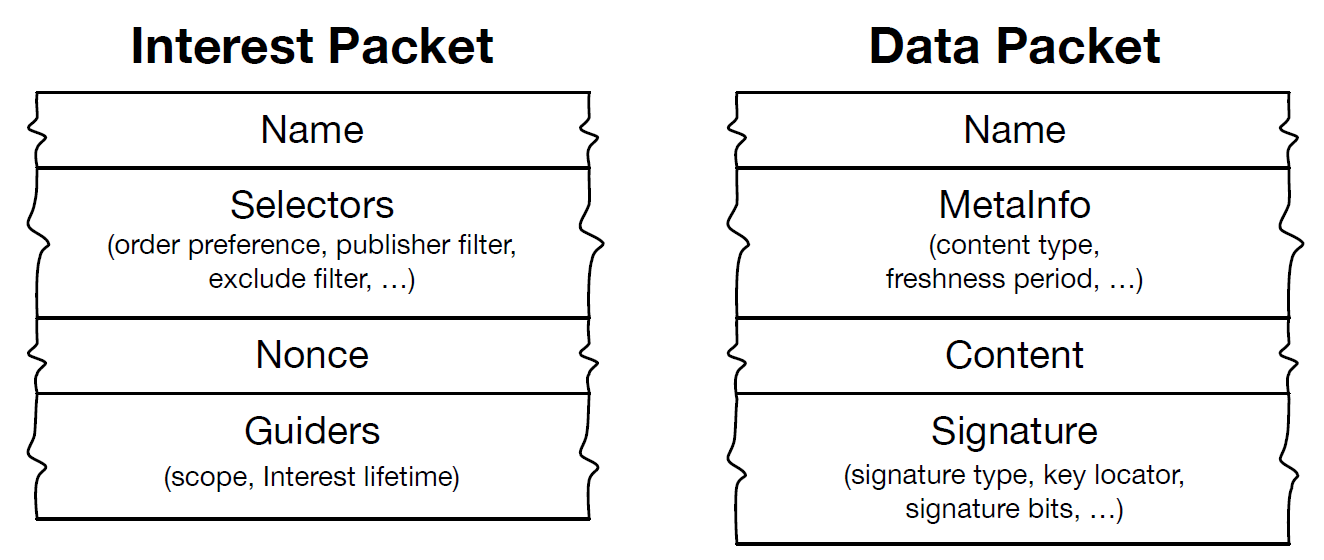
\includegraphics[width=\columnwidth]{NDN_Packets.png}
    \caption{\small Packets architecture in NDN}
    \label{fig:my_label1}
\end{figure}
  
Security in NDN is different from the current host-centric networking. Security is provided in the current internet by securing the mediums, where data and packets are transmitted. It focuses on securing the channels with different security schemes and protocols such as \cite{NGUYEN201517}\cite{661700}\cite{Fumy1998}\cite{Prentice-Hall:2000:ISP:518066}, leaving the actual packets unsecured. Within the growth of network communications, there have been needs to create more protocols to support and serve answering these communications. However, more protocols means more overhead on the network, more standardization, more configuration and less interoperability \cite{cholez:hal-00785298}. Cryptography is one solution provided a solid security, however, it also adds more overhead on the current processing. In addition, it's not a mandatory feature on a lot of systems that operate on the current host-centric networks.

In contrast, security in NDN concentrate more on securing the data packets than the channels. Contents can be located and retrieved on and from the endpoint hosts as well as the routers. NDN adapts encryption schemes for a robust security. It enforces the encryption at the production stage. Producers are compelled to sign each content with their own digital signature. Moreover, NDN provides a separate layer to encrypt every content; making this scheme a mandatory for all contents which then efficiently guarantees the integrity and authenticity for these packets regardless of how, when or where they are retrieved from \cite{Gasti2013}. Without a need for a digital certificate, NDN facilitates the security implementation by allowing the applications to manage how security is going to be executed and performed.     

   



\section{Interest Forwarding Attack (IFA)}

As previously explained, rather than a specific host’s IP address, NDN routers routes the interest packets through the network based on the content name prefixes. When an interest is created, it does not get signed by the consumer; only data packets are signed\cite{Gasti2013}. Once a router receives the interest packet it checks its CS for any existing matching data, if not then it creates a new PIT entry and then forwards the packet to upstream. This make them potential targets for an adversary to inject them with a large imprudent number of malicious interests. Using a large set of zombies on the network, an adversary can mount an excessive number of interest to overflow the PIT in the router which then interdict them to process legitimate interests. In addition, producer's content can be targeted too by swamping the content.  However, attackers cannot target a specific host. Instead, they can target a specific namespace regardless of where or which endpoints host the content. Intermediate routers also consume their memory when serving an interest packet. Therefore, not only endpoints are effected, but also the intermediate routers could be targeted too for such attack \cite{6663516}\cite{KARAMI20151262}. Figure [3].

\begin{figure} [ht]
    \centering
    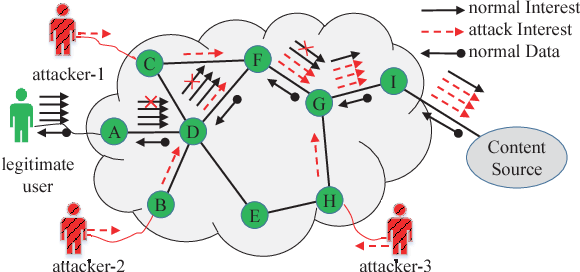
\includegraphics[width=\columnwidth]{IFA.png}
    \caption{\small Interest Flooding Attack  \cite{Xin2016ANI} }
    \label{fig:my_label2}
\end{figure}

As noted on \cite{Gasti2013}, Interest flooding attack that targets the router's PIT



acn exhaust the network by sending a huge amount of interests packets for an existing or less popular contents. That will cause a degradation on the network performance. Another type is to send a non-existing interest packet that required the the router to create a new PIT entry. The hackers by sending an excessive number of interests packets, it forces the router create fill out the memory with all those new entries created. Therefore, within a specific amount of memory, the router will not be able to serve any new new interest request as it will be declined.\cite{KARAMI20151262}       

\section{Analysis And Current Literature}
\cite{Tourani2018}
\cite{Bhattacharyya2018}
\cite{Chhetry2016}
\cite{Abdallah2015}
\cite{Chen2015}
\cite{Gasti2013}
\cite{Zhang:2014:NDN:2656877.2656887}
\cite{Compagno2013}
\cite{Dai2013MitigateDA}
\cite{6496396}
\cite{Xin2016ANI}
\cite{Chhetry2016}
\cite{Nguyen2015}
\cite{8247232}
\cite{Zhao2018}
\cite{8352953}
\cite{8452848}

\section{Discussions}

\cite{Abdallah2015}
\cite{Chen2015}
\cite{Smetters2009}
\cite{Ahlgren2012}
\cite{Universite2018}

    item Attack that targets the CS.
    item Since CS and PIT are the two structures where mostly consume the memory when serving an interest packet, they are potential for the IFA attack. 
    item Attack that targets the FIB 

\section{Conclusion}




\bibliographystyle{ieeetr}
\bibliography{Bibliography}
\end{document}
